\section{Running the pipeline}
The automated pipeline is run after the data has been obtained at the telescope. It operates on the raw ULTRACAM data, reducing it and preparing output files that are used for the Web browsing interface. The pipeline can be run anytime after the data has been recorded and is therefore useful for browsing and sharing ULTRACAM observations immediately after performing the observations, or much later, when wishing to reduce the data for a run that exists in the ULTRACAM archive.

\subsection{Prerequisites}
The pipeline is written in the Python programming language and needs a working Python environment. It is currently running on Python version 2.6.9, but has also been tested on version 2.7.6. Within the Python path, the following fairly well-known Python libraries should be installed. 
\begin{itemize}
  \item \emph{Numpy} NumPy is a well-known package for scientific computing with Python. It is available from \url{http://www.numpy.org}.
  \item \emph{Astropy} Astropy Project is a community effort to develop a single core package for Astronomy in Python and foster interoperability between Python astronomy packages. Available at \url{http://www.astropy.org/}.
  \item \emph{Matplotlib} matplotlib is a python 2D plotting library itcan be used in python scripts, the python and ipython shell. It is available at  \url{http://matplotlib.org/}
  \item \emph{Image} The Image package contains the Python Imaging Library. This library is used for loading, creating and modifying bitmap images and is used by the pipeline to create the PNG images that are used on the web pages. It can be found at \url{http://effbot.org/imagingbook/pil-index.htm}.
  \item \emph{Jinja} The Jinja2 package contains tools for creating and using template files and merging them with dynamic data. The pipeline uses this module to create the HTML files for the web site. It can be found at \url{http://jinja.pocoo.org/}.

\end{itemize}
Along with these packages, the following standard Python modules are also used by the pipeline. These packages are nearly always included by default in Python distributions.
\begin{itemize}
  \item \emph{Math} A module to perform some basic mathematical operations.
  \item \emph{Argparse} A module that aids the creation of 'command-line parameters' for the scripts in the pipeline. 
  \item \emph{Time} A module for performing time functions and operations.
  \item \emph{DateTime} A module for formatting and manageing date and calendar objects.
  \item \emph{JSON} A module for reading, writing and parsing JSON-formatted data objects. 
\end{itemize}

The source extration and flux measurement activity in the pipeline is performed by the third party software, called \emph{SExtractor}, \cite{bertin}. SExtractor can be downloaded and installed from \url{http://www.astromatic.net/software/sextractor}. If downloading and compiling from the source, there is a good guide available at: \url{http://wiki.ipb.ac.rs/index.php/SExtractor_installation}. 

In order to serve the web site, a web server is needed. Fortunately, since the web site consists purely of static files, a simple HTTP server is required. For example, an instance of the Apache web server with no server-side add-ons is perfectly adequate. 

\subsection{Installing the Python code}
The core code of the automated pipeline exists in the 'git' repository. It is therefore easy to download the code into a local directory, by typing the command: \texttt{git clone https://github.com/rashley2712/ucambuilder}.  This will create a sub directory called \texttt{ucambuilder} which will contain all of the required Python code for running the automated pipeline. Since, it is likely that you will not be running the pipeline from this directory, an important next step is to add this directory to your \texttt{PATH} and \texttt{PYTHONPATH} environment variables. 

\subsection{Config file}
It is a good idea to create a separate directory to keep configuration files and temporary files. It is also good practice to run the pipeline from this folder as it will, by default, look in the local directory for the configuration files. In this folder, you should create a few configuration files that you can modify as desired before running the pipeline. In order to get a pre-built set of configuration files, you can use a 'git' repository to create and download a folder with the default set. Typing \texttt{git clone https://github.com/rashley2712/ultracam-auto} will download the configuration files into a folder called \texttt{ultracam-auto}. 

The following files are needed as configuration files: 
\begin{itemize}
  \item \emph{ucambuilder.conf} This is the pipeline's main configuration file and is used to store the parameters that specify where the pipeline should look for the raw data, where it should write the output files, etc. This is discussed in more detail in the next section of this document. 
  \item \emph{default.sex} Is the configuration file that is loaded when {SExtractor}.  This files contains many parameters that instructs {SExtractor} on how to perform the source extraction and flux calculation in the image. More details on these parameters can be found in the {Sextractor} User Manual \footnote{\url{https://www.astromatic.net/pubsvn/software/sextractor/trunk/doc/sextractor.pdf}}. 
  \item \emph{default.param} This file lists the columns that we want {SExtractor} to include in the output catalog. These columns are read by the automated pipeline in order to build up the master catalog. We need {SExtractor} to output flux measurements, pixel coordinates and measurement flags. Generally these parameters do not need to be edited. 
  \item \emph{default.conv} This file defines the profile of the convolution filter that {Sextractor} applies to the image before source extraction. 
\end{itemize}

\subsection{ucambuilder.conf}
A sample of the main configuration file for the automated pipeline is shown below.
\lstset{basicstyle=\scriptsize}
\begin{lstlisting}
DEBUG   1       # The debug level to be used by the various scripts. Can be 1, 2, 3
SITE_PATH       /storage/astro2/www/phrnaw/sitedev      # The path to the website
ULTRACAMRAW     /storage/astro1/phsaap/ultracam/raw_data        # Path to the Ultracam raw data
WRITE_FITS      0       # Write a fits file or not?
WRITE_JSON      1       # Write a fits file or not?
KEEP_TMP_FILES  0       # Keep the temporary (sextractor) files?
RUNTEMPLATE     /storage/astro2/www/phrnaw/sitedev/sitecode/runxxx.jinja
DAYTEMPLATE     /storage/astro2/www/phrnaw/sitedev/sitecode/day-xxxx-xx-xx.jinja
MINPIXELDISTANCE        10
RUNINFO         /storage/astro1/phsaap/ultracam/logs/ultra.json
WORKINGDIR      /storage/astro2/phrnaw/workingdir
ROOTURL         http://deneb.astro.warwick.ac.uk/phrnaw/sitedev/
SEX_MAGNITUDE   FLUX_AUTO
COMPARISON_THRESHOLD    95
\end{lstlisting}

These parameters should be modified before running the pipeline.

\begin{itemize}
	\item \texttt{SITE\_PATH} Specifies where the document root for the web folder is. The pipeline will write the HTML and JSON files to this folder. For each date in the archive, the pipeline will create sub-directories in the format \texttt{YYYY-MM-DD}. A web server should be configured to serve HTTP requests from this folder. 
	\item \texttt{ULTRACAMRAW} This should point to the root folder where the raw ULTRACAM data is stored. Within this folder there will be sub-folders corresponding to each date on which the ULTRACAM was active. These folders will contain \texttt{.dat} and \texttt{.xml} files corresponding to each run recording during that observing night.  
	\item \texttt{ROOTURL} Specifies where the \texttt{SITE\_PATH} is accessed in URL space. In other words, this is the URL to the web site that is configured to serve files from the \texttt{SITE\_PATH} folder. 
	\item \texttt{WORKINGDIR} This is a folder where the pipeline will place temporary working files used to connect the intermediate stages of the pipeline. They are not required for the web version of the output, but they can be useful to debug and diagnose the running of the pipeline to better understand how it has arrived at the final results. 
	\item \texttt{RUNINFO} The location of file that contains important meta-data about the ULTRACAM archive, such as run numbers, durations, comments and RA and DEC locations of the field. This data is used to add information to the web pages and to aid the astrometry solution. 
	\item \texttt{RUNTEMPLATE} \& \texttt{DAYTEMPLATE} Specify the location of the HTML template files that are used to create the final versions that for the web pages. 
	\item \texttt{SEX\_MAGNITUDE} This parameter instructs the pipeline which value of the flux estimate produced by {SExtractor} to use for the brightness measurement of the object in the master catalog. Possible values are \texttt{FLUX\_AUTO, FLUX\_APER, MAG\_AUTO \& MAG\_APER}.
	\item \texttt{MINPIXELDISTANCE} The minimum pixel difference used to allow a match of an object across the 3 channels. If the object is more than this distance from the same object in a different channel, then it is treated as a new object.
	\item \texttt{COMPARISON\_THRESHOLD} The pipeline tries to find an object that can act as a comparison object for the other objects in the field. It does this by performing a statistical test for consistency of the differential flux measurements of the top 20 brightest objects in the field and then choosing the brightest of the objects that has the lowest standard deviation of the mean with another object in the field. This comparison is not used during the data reduction portion of the pipeline, but it is automatically selected as the default comparison object when the web browser session is first loaded. This parameter defines the minimum percentage of the run that the object has to persist on in order to be considered as a comparison object. 
\end{itemize}

\subsection{Producing the output for a particular run}

\subsubsection{runbuilder.py}

The quickest way to create the output for a particular run is to use the macro-script, \texttt{runbuilder.py}. This script chains together the various stages of the pipeline to produce the HTML and JSON output required to view a particular run. It runs each of the following scripts in the pipeline in turn: \texttt{objectdbcreator.py}, \texttt{postprocessor.py}, \texttt{wcssolver.py}, \texttt{mergeobjects.py} and \texttt{create\_html.py}.

\texttt{runbuilder.py} takes the following command line parameters:
\begin{itemize}
  \item \texttt{runName} This is a path to the \texttt{.xml} and \texttt{.dat} for a specific run and is specified in the format \texttt{YYYY-MM-DD/runXXX}  (for example \texttt{2013-07-21/run011}).
  \item \texttt{-n[n] --numframes [n]} Specifies the number of frames you would like the script to process. The default is all of the frames in the run. Making this number smaller is useful for running a quick test. For example, \texttt{-n100} will run through 100 frames only.
  \item \texttt{-c[filename] --configfile [filename]} Allows you to specify an alternative configuration file. By default, the script will look for a file called ``ultracam.conf" in the local directory. 
  \item \texttt{-w} Use this switch to disable the astrometric solution step in the pipeline. This can be used to save time when we have a run where we do not expect to find an astrometric solution. This occurs when the run has only two or three objects on it and/or the windowed portions of the CCD are very small.  
  \item \texttt{-v[version] --version [version]} Specify a unique string to act as an identifier for an alternate version of the output of the pipeline. This can be used if we want to re-run the pipeline, but with different SExtractor parameters and compare the outputs. The resulting web pages will have a URL that has this version string appended.    
\end{itemize}

For more information on the output of \texttt{runbuilder.py} see the section below, describing 'Output while running'.

When \texttt{runbuilder.py} has completed, it will display the URL to the output run in the terminal window. This URL can then be copied into a web browser's location bar in order to access the results of the reduction.

\subsubsection{objectdbcreator.py}

This is the most important script in the automated pipeline. It takes the raw image data in the ULTRACAM archive and sends it to SExtractor for processing. Based on the SExtractor output, it compiles and maintains a list of objects across all of the frames and each of the channels. These are given as three output catalogs when the script finishes running. 

\texttt{objectdbcreator.py} takes the following command line parameters:
\begin{itemize}
  \item \texttt{runName} This is a path to the \texttt{.xml} and \texttt{.dat} for a specific run and is specified in the format \texttt{YYYY-MM-DD/runXXX}  (for example \texttt{2013-07-21/run011}).
  \item \texttt{-d[n] --debug [n]} Use this parameter to determine how much output you would like to see while the program is running. There are 3 debug levels, \emph{1} is silent (except for errors) and is the default debug level; \emph{2} shows general progress of the pipeline; \emph{3} shows detailed info to help with debugging. Note that the default is `silent' and therefore, unless there are errors, you will not see anything on the command line and a long run through the data could last an hour or more. It is recommended that you use \texttt{-d2} in most cases. 
  \item \texttt{-n[n] --numframes [n]} Specifies the number of frames you would like the script to process. The default is all of the frames in the run. Making this number smaller is useful for running a quick test. For example, \texttt{-n100} will run through 100 frames only.
   \item \texttt{-s[n] --startframe [n]} Specifies which frame to start at. The default is frame 1 (the first frame in the run). 
  \item \texttt{-c[filename] --configfile [filename]} Allows you to specify an alternative configuration file. By default, the script will look for a file called \texttt{ultracam.conf} in the local directory. 
  \item \texttt{-C[r,g,b] --channels [r,g,b]} Which channels to operate the pipeline over. By default, the script will process all three channels, namely, r, g, and b. This parameter allows you to specify a subset of these channels. For example, you could omit the processing of the `green channel' by passing in \texttt{-Crb}. 
  \item \texttt{-p --preview} Specifying this parameter enables a preview window for each frame and each channel using \emph{Matplotlib}. This allows you to see each frame as it is being processed. The colour palettes match the channel, red for r, green for g and blue for b. The preview window also draws a green circle around each object that SExtractor has identified on that particular frame. Warning: This preview slows down the pipeline significantly so should only be used for information and debugging purposes. 
  \item \texttt{-t[n] --sleep [n]} Time to pause (in seconds) between the processing of each frame. Useful for debugging in `preview' mode. 
  \item \texttt{-r --crop} For `preview' mode, crop the windows to show only the areas that were not masked in the original data. Useful for runs where the windows are fairly small. 
  \item \texttt{-v[version] --version [version]} Specify a unique string to act as an identifier for an alternate version of the output of the pipeline. This can be used if we want to re-run the pipeline, but with different SExtractor parameters and compare the outputs. The resulting web pages will have a URL that has this version string appended.    

\end{itemize}

\subsubsection{Output while running}
If the \texttt{--debug} option is left to the default value of \texttt{1} then the output will be mostly \emph{silent} with only errors appearing in \texttt{stdout}. This mode is designed for use during the running of the pipeline across a complete night where we want to suppress a lot of the output. If you are running \emph{objectdbcreator.py} in standalone mode, then \texttt{-d2} is recommended. 

The output of the script with \texttt{-d2} set looks like this:

\begin{lstlisting}
[10:31:25] 00:10:22 Frame: [1681,1681 87%] MJD:56495.1395466 r:1899 g:1030 b:551 
[10:31:27] 00:10:19 Frame: [1682,1682 87%] MJD:56495.1396132 r:1900 g:1030 b:551 
[10:31:29] 00:10:17 Frame: [1683,1683 87%] MJD:56495.1396799 r:1900 g:1030 b:551 
[10:31:32] 00:10:14 Frame: [1684,1684 87%] MJD:56495.1397465 r:1900 g:1030 b:552 
\end{lstlisting}

Where, 
\begin{itemize}
  \item \texttt{[10:31:25]} is the current time, in HH-MM-SS format;
  \item \texttt{[00:10:22]} is the estimated time remaining, in HH-MM-SS format, until this stage of the pipeline has completed. ;
  \item \texttt{Frame:[1681, 1681 87\%]} The first number is the absoluted frame number being processed (starts at first frame of the run = 1), the second number is the relative frame being processed (different if the start frame was not = 1), and the percentage completed;
  \item \texttt{MJD:56495.1395466} is the MJD for this frame;
  \item \texttt{r:1899 g:1030 b:551} shows the number of objects being tracked in each of the r, g, b channels.
\end{itemize}

\subsubsection{postprocessor.py}
The second stage of the pipeline performs a filtering of the data as described in section \ref{sect:filtering}. It also creates output catalog files containing an ordered list of the pixel coordinates and fluxes for the brightest objects in the field for each of the r, g, b channels. These can be used as inputs to the Astrometry.net software for the solving of the WCS coordinates for the field. 

\texttt{postprocessor.py} takes the following command line parameters:
\begin{itemize}
  \item \texttt{runName} This is a path to the \texttt{.xml} and \texttt{.dat} for a specific run and is specified in the format \texttt{YYYY-MM-DD/runXXX}  (for example \texttt{2013-07-21/run011}).
  \item \texttt{-d[n] --debug [n]} Use this parameter to determine how much output you would like to see while the program is running. There are 3 debug levels, \emph{1} is silent (except for errors).
  \item \texttt{--xyls} UIse this switch to create the output catalogs for Astrometry.net. The script will create three catalogs (r, g, b) in FITS format for input into the Astrometry.net software.
  \item \texttt{-c[filename] --configfile [filename]} Allows you to specify an alternative configuration file. By default, the script will look for a file called \texttt{ultracam.conf} in the local directory. 
  \item \texttt{-v[version] --version [version]} Specify a unique string to act as an identifier for an alternate version of the output of the pipeline. This can be used if we want to re-run the pipeline, but with different SExtractor parameters and compare the outputs. The resulting web pages will have a URL that has this version string appended.    
\end{itemize}

\subsubsection{wcssolver.py}
This script configures and runs the WCS solving step of the pipeline. It is really just a script that prepares and runs the Astrometry.net package. 

\texttt{wcssolver.py} takes the following command line parameters:
\begin{itemize}
  \item \texttt{runName} This is a path to the \texttt{.xml} and \texttt{.dat} for a specific run and is specified in the format \texttt{YYYY-MM-DD/runXXX}  (for example \texttt{2013-07-21/run011}).
  \item \texttt{-d[n] --debug [n]} Use this parameter to determine how much output you would like to see while the program is running. There are 3 debug levels, \emph{1} is silent (except for errors).
  \item \texttt{-f --forcesolve} The script usually checks the \texttt{WORKINGDIR} to see if a WCS solution for this field already exists and will skip Astrometry.net if it finds one. Use this switch to force the script to call Astrometry.net even if a solution already exists.
  \item \texttt{-c[filename] --configfile [filename]} Allows you to specify an alternative configuration file. By default, the script will look for a file called \texttt{ultracam.conf} in the local directory. 
  \item \texttt{-v[version] --version [version]} Specify a unique string to act as an identifier for an alternate version of the output of the pipeline. This can be used if we want to re-run the pipeline, but with different SExtractor parameters and compare the outputs. The resulting web pages will have a URL that has this version string appended.    
\end{itemize}

\subsubsection{mergeobjects.py}
This script loads the three separate catalogs and performs a merge of the objects into one 'master' catalog. It also writes the JSON files that are placed in the web server's directory, ready to be loaded by the HTML and Javascript for viewing the results. 

\texttt{mergeobjects.py} takes the following command line parameters:
\begin{itemize}
  \item \texttt{runName} This is a path to the \texttt{.xml} and \texttt{.dat} for a specific run and is specified in the format \texttt{YYYY-MM-DD/runXXX}  (for example \texttt{2013-07-21/run011}).
  \item \texttt{-d[n] --debug [n]} Use this parameter to determine how much output you would like to see while the program is running. There are 3 debug levels, \emph{1} is silent (except for errors).
  \item \texttt{-c[filename] --configfile [filename]} Allows you to specify an alternative configuration file. By default, the script will look for a file called \texttt{ultracam.conf} in the local directory. 
  \item \texttt{-v[version] --version [version]} Specify a unique string to act as an identifier for an alternate version of the output of the pipeline. This can be used if we want to re-run the pipeline, but with different SExtractor parameters and compare the outputs. The resulting web pages will have a URL that has this version string appended.    
\end{itemize}

\subsubsection{create\_html.py}
This script takes the run meta-data and merges this with the HTML templates stored in \texttt{RUNTEMPLATE} to create the HTML files used for web browsing. 

\texttt{create\_html.py} takes the following command line parameters:
\begin{itemize}
  \item \texttt{runName} This is a path to the \texttt{.xml} and \texttt{.dat} for a specific run and is specified in the format \texttt{YYYY-MM-DD/runXXX}  (for example \texttt{2013-07-21/run011}).
  \item \texttt{-d[n] --debug [n]} Use this parameter to determine how much output you would like to see while the program is running. There are 3 debug levels, \emph{1} is silent (except for errors).
  \item \texttt{-c[filename] --configfile [filename]} Allows you to specify an alternative configuration file. By default, the script will look for a file called \texttt{ultracam.conf} in the local directory. 
  \item \texttt{-v[version] --version [version]} Specify a unique string to act as an identifier for an alternate version of the output of the pipeline. This can be used if we want to re-run the pipeline, but with different SExtractor parameters and compare the outputs. The resulting web pages will have a URL that has this version string appended.    
\end{itemize}

\subsection{Producing the output for a full night's observing}
There is a macro Python script called \texttt{daybuilder.py} that runs the pipeline on all of the runs in any particular night. The script effectively runs the \texttt{runbuilder.py} script for all of the runs found on the date specified. It also produces a summary web page showing all of the runs with descriptions and thumbnails, making navigating the reductions for that night quite easy.

\texttt{daybuilder.py} takes the following command line parameters:
\begin{itemize}
  \item \texttt{runDate} The date for the night of interest. Specified in the format \texttt{YYYY-MM-DD}.
  \item \texttt{-d[n] --debug [n]} Use this parameter to determine how much output you would like to see while the program is running. There are 3 debug levels, \emph{1} is silent (except for errors).
   \item \texttt{-c[filename] --configfile [filename]} Allows you to specify an alternative configuration file. By default, the script will look for a file called \texttt{ultracam.conf} in the local directory. 
  \item \texttt{-r --buildruns} Build the run output for each run (if no existing output found).
  \item \texttt{-f --forcebuildruns}  Force build of each run (even if existing data is found).
\end{itemize}
 

\section{Using the archive} 

\subsection{Night summary page}
Once the pipeline has been run, the HTML and JSON files will be ready to view through a web. You can access the output of any night of observing by entering a URL into the web browser of the following format, \url{http://deneb.astro.warwick.ac.uk/phrnaw/sitedev/YYYY-MM-DD/index.html} where you need to substitute the \texttt{YYYY-MM-DD} portion of the URL with the date in question. This will load an HTML page showing you \emph{all} of the runs that occured during that night. This list will include aquisition runs, biases and flat fields as well as the science runs. The page shows a thumbnail of each run along with a description of the target object, RA and DEC, run duration and the comments entered by the observer at the telescope. Clicking on the run thumbnail will take you to the web page for that particular run. 

\begin{figure}
  \centering
  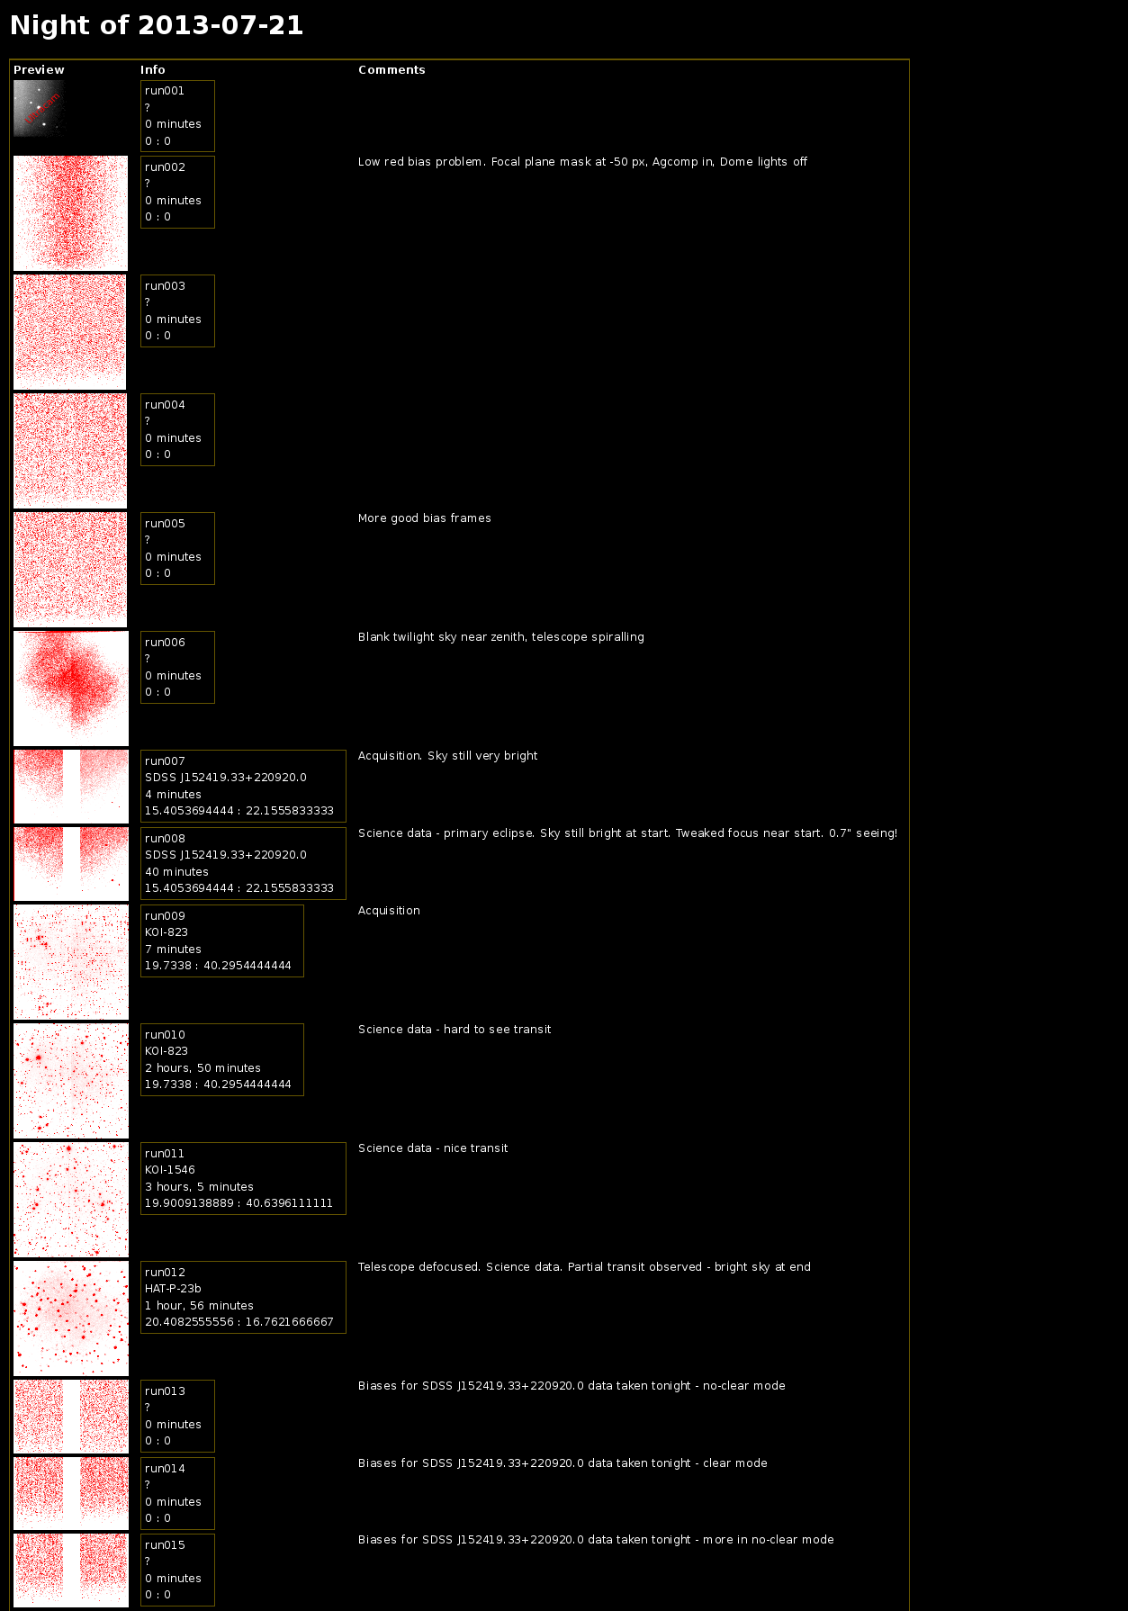
\includegraphics[width=120mm]{images/index_webpage.png}
  \caption{Example of the web page summarising a full night's observing.}
  \label{fig:indexwebpage}
\end{figure}

\subsection{Run page}
When viewing the web page for a particular run, the user can navigate the light-curves for all of the objects identified by the pipeline. Interaction with the data in the page is through the mouse and keyboard. Many of the actions are triggered by a single key press. There are also tickboxes, and radio buttons that allow the selection of various options. 

\subsubsection{Page loading process}
The page has three main components, HTML, Javascript and JSON. The HTML and Javascript define the page structure and the interactions that can occur, while the JSON contains the reduction data for all of the objects in the run. The JSON datafile is requested from the web server as soon as the HTML and Javascript has finished loading (within 1 second or so). For long runs with many (>20) objects, this file can be quite large and will take some time to download. Depending on the data size and the speed of the internet connection, this download could take up to a minute or more, although in most cases it is usually completed in a few seconds. The status window at the top of the page will give an indication of when this data has completed the download. The request for the JSON data is made using an 'asynchronous' call and this means that the page is still working and some interactions can take place, like choosing the base image for example, but since to main data has not yet arrived, it won't be possible to display a light-curve.  
r
\subsubsection{Selecting a base image}
The pipeline produces a deep image for each channel (r, g, b) based on stacking all of the individual frames captured by ULTRACAM. The page loads all three images in the background and, by default, displays the 'green' channel initially. Switching between these images can be performed by pressing the \texttt{r}, \texttt{g} and \texttt{b} keys on the keyboard. You can also switch these images by slecteing either the \texttt{Red},  \texttt{Green} or \texttt{Blue} of the \texttt{Base Image} radio options found below the image itself.

\subsubsection{Viewing a light-curve}
The quickest way to view a light-curve of any particular object is to simply click on the object with the mouse. If the object has been identified by the pipeline and there are sufficient data to display, then a light curve for this object will appear in the panel below the radio buttons and checkboxes on the page. While moving the mouse over the base image, the cursor that displays the $(x, y)$ coordinates (or the $(RA, DEC)$ coordinates will display a green background if the object underneath it has the required data for a light-curve.

\subsubsection{Object markers and Object labels}
Each object that has been identifiedby the pipeline has a unique identifier in the master catalog. In order to view these IDs, you can toggle the object 'labels' on and off. This is done by pressing the (letter 'l') \texttt{l} key, or clicking the \texttt{Show labels} checkbox. This will draw lavels next to each object identified by the pipeline that has photometry available in the channel that is currently selected for the base image. If you want to see each of the identified objects shown as a circle centred on each object, rather than a label, then pressing the \texttt{m} key or checking the \texttt{Show circles} check box will toggle the drawing of circles of radius 15 pixels around each object.   

\subsubsection{Selecting a comparison star}
During the final stage of the pipeline, a test is performed on the brightest objects to see if any can act as comparison stars for the run. The test takes into account the standard deviation of the star's flux measurments in comparison to the other bright stars in the field. If an object is deemed to be significantly 'constant' enough, then it is flagged as a potential comparison star. When the data has finished loading, this comparison star (if one exists) is selected. The test is performed independantly for each channel. It is possible for the user to select a different comparison star for each channel. This is done by selecting the object and pressing the key \texttt{c}. When the object is selected, a black diamond is drawn around the object. When the object is selected as the comparison object, this diamond will change to a square. To indicate that a comparison object for this channel has now been selected, the \texttt{Comparison objects} status area will now indicate the Object ID, or the comparison and the the light-curve of the comparison object will be displayed below the light-curve of the target object.

\begin{figure}
  \centering
  \setlength{\fboxrule}{1pt}

  \fbox{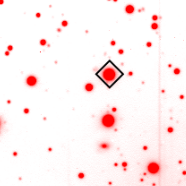
\includegraphics[width=40mm]{images/selectedobject.png}}
  \fbox{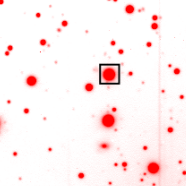
\includegraphics[width=40mm]{images/selectedcomparison.png}}
  \caption{Selecting an object to act as the comparison. First select the object, then press the \texttt{c} key on the keyboard. The cursor will change from a diamond to a square, indicating that this object is now the comparison for this channel ('r' in this case).}
  \label{fig:selectcomparison}
\end{figure}  

\subsubsection{Re-scaling the light curve}
The vertical axis on the light curve of the target object can be adjusted to adapt to the dynamic range of the flux measurements. By default, when the page is loaded, the light-curve of the target is calculated as the ratio of the flux of the target object to the flux of the comparison object. This value is then also normalised to fill the range from $[0 to 1]$. The normalisation step can be disabled by unchecking the \texttt{Normalise the chart} check box on the web page. Feedback from early users of this page has suggested moving to a magnitude ($log_{10}$) scale by default. This will be implemented in the next iteration of the pipeline. In order to view the light-curve in raw flux measurements, rather than as a ratio with the comparison, then the \texttt{Use comparison} check box can be unchecked.

\begin{figure}
  \centering
  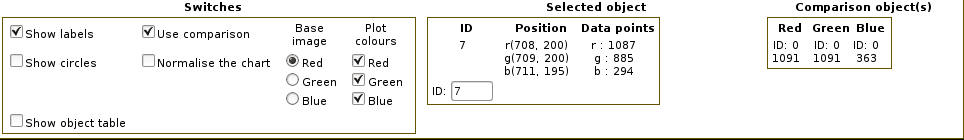
\includegraphics[width=140mm]{images/webcontrols.png}
  \caption{Sample of the control panel of the run web page. This screenshot shows some of the radio buttons and checkboxes available to the user to manipulate the displayed light-curves. }
  \label{fig:webcontrols}
\end{figure}  

\subsubsection{Plotting the position of the object}
Once an object is selected, it is possible to produce a chart of the object's $(x, y)$ pixel position during the duration of the run. Pressing the \texttt{p} key will produce this plot, which 

\subsubsection{Exporting to a CSV file}
Once a light-curve is displayed, pressing the \texttt{e} key will start the download of a comma-seperated value (CSV) file. Most browsers will allow you to rename this file and save to the local disk. The data saved will reflect the light-curve that is currently displayed. ie. If the current light curve is displaying normalised values, then these are the ones that will be exported in the CSV file.

%\subsection{Walkthrough - spotting an exoplanet transit}
